\documentclass{article}

\author{Pedro Henrique Limeira da Cruz}
\title{Trabalho Final - ES101}

\usepackage[margin=0.8in]{geometry}
\usepackage{indentfirst}
\usepackage{fancyhdr}
\usepackage{tcolorbox}
\usepackage{graphicx}
\usepackage{amsmath}
\usepackage{amssymb}

% Create a new command to be used in the align environment in multiple line equations do only the last equation is numbered  
\newcommand{\n}{\nonumber \\ }
\makeatletter
\let\inserttitle\@title
\makeatother
% Set the style of the page 
\pagestyle{fancy}
\fancyhf{}
\rhead{Pedro Henrique L. da Cruz}
\lhead{\inserttitle}
\rfoot{Page \thepage}

\usepackage{hyperref}
\hypersetup{
    colorlinks=true,
    linkcolor=black,
    filecolor=black,
    urlcolor=black,
}

% Begin the Document 
\begin{document}

    \maketitle
    \thispagestyle{empty}

    % Add the image inside a figure in as the first page
    \begin{figure}[h]
        \begin{center}
            
\includegraphics[scale = 0.15]{/Users/pedrocruz/Documents/UNICAMP/ES101/ES101 - Robotic Arm/img/unicamp.png}
        \end{center}
    \end{figure}

    % Change to the Next page 
    \newpage

    \section[Rev. Dinâmica]{Revisão de Dinâmica}

        \subsection{Cinética Plana de Corpos Rígidos}

            \subsubsection[Intro]{Introdução}
                A cinética de corpos rígidos trata das relações entre as forças externas sobre um corpo e seu movimento resultante (que é composto pela rotação e translação). Para a abordagem a seguir, o
                corpo apresenta um \textbf{CG} (Centro de Massa / Centro de gravidade), de maneira que todas as forças que atuam sobre o corpo atuam sobre ele.

                No Total, para caracterizar totalmente o movimento de um corpo em um plano são necessárias 3 equações, sendo elas:
                \begin{enumerate}
                    \item Somatório de Forças no Eixo $X$
                    \item Somatório de Forças no Eixo $Y$
                    \item Somatório de Momentos Gerais
                \end{enumerate}

                Além disso, para analisarmos as formas e momentos supracitados, também é necessário (em primeiro lugar) a análise de \emph{DCL} (Diagrama de Corpo Livre).

            \subsubsection[Eq. Gerais do Mov.]{Equações Gerais do Movimento}

                Como havia sido dito anteriormente, para descrevermos por completo o movimento de um corpo em um plano é necessário 3 equações, sendo duas de forças e uma de momento. Sendo elas:
                \begin{align}
                    \sum \vec F = m \cdot \vec{\bar a} = \dot{\vec{G}}_{CG} \label{eq:SomaDasForcasCg} \\
                    \sum \vec M_G =  I \cdot \vec{\bar\alpha} = \dot{\vec{H}}_{CG} \label{eq:soma_dos_momentos_cg}
                \end{align}

                Explorando mais as equações acima, temos que:
                \begin{itemize}
                    \item $\bar a$: Aceleração linear do centro de massa;
                    \item $\alpha$: Aceleração angular do centro de massa;
                    \item $\bar I$: Momento de inércia do corpo (i.e a medida de resistência à variação na velocidade de rotação devido à distribuição de massa em torno do CG)
                    \item $\dot{\vec{G}}$: A variação no tempo da \emph{Quantidade de Movimento Linear} no \emph{CG}
                    \item $\dot{\vec{H}}$: A variação no tempo da \emph{Quantidade de Movimento Angular} no \emph{CG}
                \end{itemize}

                É válido ressaltar, ainda, que a \emph{Quantidade de Movimento Linear} e a \emph{Quantidade de Movimento Angular} são grandezas vetoriais que é definida pelo produto entre a velocidade (linear e angular)
                com a inércia (i.e a massa e a momento de inércia). E são de suma importância pois tem relação direta com força e momento (como visto anteriormente).


            \subsubsection[Eq. Alternativa do Momento]{Equação Alternativa do Momento}

                A fórmula \ref{eq:SomaDasForcasCg} modela a soma de momentos somente quando estamos analisando o sistema tomando como referencial o centro de gravidade \emph{CG}. Isso,
                entretanto, nem sempre é possível, tendo em vista a complexidade que algumas topologias assumem, o que tornaria inviável fazer sua análise. Há, todavia, uma forma alternativa de
                modelarmos o sistema, considerando um ponto $P$ arbitrário, a uma distância $d$ conhecida:
                \begin{align}
                    \sum \vec M_P = \bar I \cdot \alpha + m \bar a d \label{eq:soma_dos_momentos_ponto_p}
                \end{align}

                Onde $a$ é a aceleração linear no centro de gravidade. 
                
                Ao analisarmos bem a equação, podemos observar que ela nada mais é do que o momento no próprio centro de gravidade, dado pela parcela $\bar I \alpha$, somado ao momento (também
                chamado de torque) que a força resultante ($\sum F = m \bar a$) gera no ponto $P$ a uma distância $d$ do CG em análise.

            \subsubsection[Sis. de Corps. Interligados]{Sistemas de Corpos Interligados}
                
                Em casos mais complexos, a principal topologia que encontramos é a de corpos extensos interligados. Um clássico exemplo disso é o problema do carro com pêndulo, onde temos um carro
                (primeiro corpo) conectado a uma mola e a uma parede, que possui um pêndulo (segundo corpo) com seu  pivô de rotação localizado no \emph{CG} do carrinho.

                Para problemas assim, temos a generalização das fórmulas, como sendo:

                \begin{align}
                    \sum \vec F = \sum m \vec{\bar a} \label{eq:soma_das_forcas_corps_interligados} \\
                    \sum \vec{M}_P = \sum \bar I  \alpha + \sum m \vec{\bar a} d \label{eq:soma_dos_momentos_corps_interloigados}
                \end{align}

                A equação \ref{eq:soma_dos_momentos_corps_interloigados} pode, ainda, ser reescrita considerando a notação da \emph{Teoria dos Eixos Paralelos}, que é dada por:
                
                \begin{align}
                    \begin{cases}
                        \sum \vec{M}_P &= I_P \alpha \\ 
                        I_P &= \bar I + m \bar r^2
                    \end{cases}
            \end{align}

            Isso é verdade pois $m \alpha \bar r^2 = m (\alpha \bar r) \bar r = m \bar a \bar r $, que podemos ver ser igual à equação \ref{eq:soma_dos_momentos_ponto_p}

        \subsubsection[Aplicação]{Aplicação}

            \textbf{EXEMPLO 1 - } O exemplo mais clássico para a aplicação de todos os conceitos vistos é o problema do carro com pêndulo, que é o que veremos agora:


            No geral, iremos seguir os seguintes passos:
            \begin{enumerate}
                \item Diagrama de corpo livre: A primeira coisa que devemos fazer em qualquer problema de dinâmica e Vibrações é desenhar o \emph{DCL}(Diagrama de corpo livre).
                \item Listagem dos Dados conhecidos: Em seguida, é de suma importância listarmos todos os dados que possuímos sobre o problema.
                \item Equações do Movimento: Nesse passo precisamos primeiramente identificar se estamos lidando com corpos interligados (e por conseguinte utilizaremos as equação 
                \ref{eq:soma_das_forcas_corps_interligados} e \ref{eq:soma_dos_momentos_corps_interloigados}), ou se estamos lidando com corpos simples (e então usaremos as equações 
                \ref{eq:SomaDasForcasCg}, \ref{eq:soma_dos_momentos_cg} e \ref{eq:soma_dos_momentos_ponto_p})
            \end{enumerate}



    \section{Introdução à Vibrações}

            Vibração é o movimento repetitivo, que pode ser:
            \begin{itemize}
                \item Desejado
                \item Não Desejado
            \end{itemize}

            Além disso, a vibração pode ser vista não somente como um movimento, mas também como a troca entre \emph{energia potencial} (e.g potencial elástico, potencial gravitacional, etc) e
            \emph{energia mecânica}.

    \section{Vibrações livres não Amortecidas - 1 DOF}

            Primeiramente, é importante entendermos que definimos os tipos de vibrações de acordo com certas características, sendo elas:
            \begin{enumerate}
                \item Graus de Liberdade: A depender do número de coordenadas que são necessários para a modelagem completa do movimento.
                \item Amortecimento: A depender se há o amortecimento, i.e a dissipação de energia de alguma forma (e.g um amortecedor de fluidos, atrito, ...). E pode ser classificado como:
                    \subitem Amortecido: Quando ocorre a dissipação de energia;
                    \subitem Não-Amortecido: Quando não ocorre a dissipação de energia e, por conseguinte, o movimento não para.

                \item Liberdade de Vibração: Que se refere à presença ou não de forças externas atuando no \emph{sistema} \footnote{Importante ressaltar que a definição do sistema implica na sua classificação}.
                    \subitem Vibração Livre: Não há forças externas atuando no sistema;
                    \subitem Vibrações Não-Livres: Há forças externas.

                \item Parâmetros Concentrados: Um sistema é dito de parâmetros concentrados quando os corpos que o integra são representados por corpos concentrados, e.g massas e molas.
            \end{enumerate}


            \subsection{Sistema Massa-Mola}

                Um sistema massa mola, como descrito na imagem abaixo, assim como o nome sugere, é composto por:
                \begin{itemize}
                    \item Massa  de valor $m$
                    \item Mola de rigidez $k$
                    \item Gravidade \footnote{Importante ressaltar que nesse sistema estamos incluindo a terra (e por conseguinte suas ações na massa, e por isso continua sendo um problema de
                    \emph{Vibração Livre})} $g$
                \end{itemize}

                Agora, para realizarmos a análise de vibrações desse problema, iremos seguir as seguintes etapas:
                \begin{enumerate}
                    \item Definição de Coordenadas
                    \item Diagrama de Corpo Livre
                    \item Equações de Movimento
                \end{enumerate}

                \subsubsection*{1º Passo - Definição de Coordenadas}

                    Algo muito importante de se perceber quando estamos lidando com problemas com molas (principalmente aqueles de massa-mola na vertical) é que existem dois principais pontos de
                    interesse de serem definidos no espaço, sendo eles:
                    \begin{itemize}
                        \item Posição sem deformação da mola: Isso é, posição no espaço onde a mola não exerce força alguma, devido ao fato de que a força elástica $F_e$ é dada por $F_e = k \delta$
                        \item Posição onde há equilíbrio entre a força elástica e as demais (principalmente força peso $F_p$)
                    \end{itemize}

                    Levando isso em consideração, o jeito mais fácil de lidar com esse dois pontos é criando dois eixos de coordenadas, cada um contendo seus respective zeros nesses ponto. 
                    Portanto, o primeiro passo que precisamos fazer é definir uma coordenada $y$ a qual possui zero zero no ponto onde a mola
                    \textbf{NÃO} está deformada, \emph{i.e} ela está com seu tamanho normal.
                    Em seguida, definimos nosso segundo eixo de coordenadas $x$ contendo seu $x_0$ no ponto onde as forças peso e elástica se anulam.

                    \begin{figure}[h]
                        \centering
                        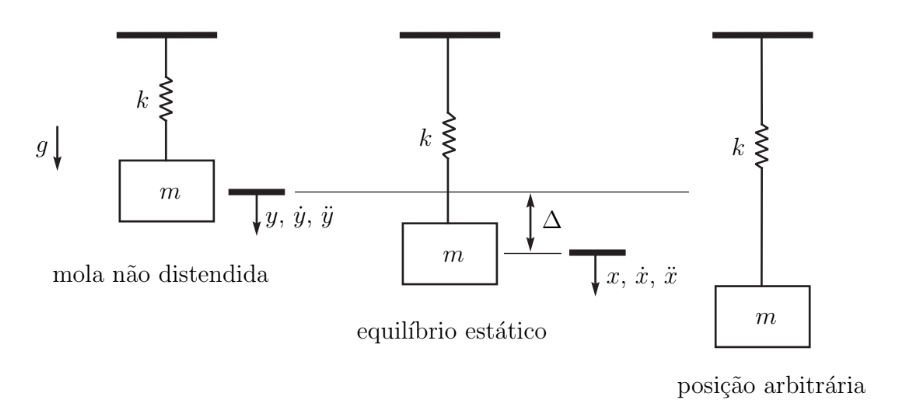
\includegraphics[width=.7\linewidth]{imgs/sis_mass_mola_1.png}
                        \caption{Coordenadas para o Problema Massa-Mola na Vertical}
                    \end{figure}

                    Esses dois eixos de coordenadas distintos, como veremos mais para frente, facilitam bastante os nosso cálculos de equação de movimento.
                    A partir disso, já temos definidos todos os pontos de interesse, e podemos prosseguir para o diagrama de corpo livre \emph{DCL}.

                \subsubsection*{2º Passo - Diagrama de Corpo Livre \emph{(DCL)}}

                    Para fazermos o DLC, precisamos primeiro considerar o bloco em uma posição arbitrária. Como já definimos os dois eixos de referência para baixo, iremos considerar o bloco em um
                    ponto tal que $x,y>0$, para facilitar os cálculos.

                    \begin{figure}[h]
                        \centering
                        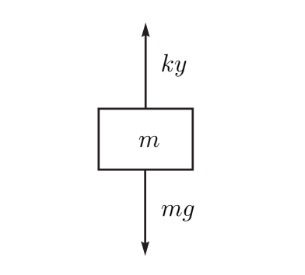
\includegraphics[width=.3\linewidth]{imgs/sis_mass_mola_1_dcl.png}
                        \caption{\emph{DCL} básico do sistema massa-mola}
                    \end{figure}

                    A partir disso, podemos fazer o DCL, que possui algumas características, que possuem o acronym (em inglês) \emph{B.R.E.A.D}:
                    \begin{itemize}
                        \item \emph{Body} : Precisa representar o corpo que está sendo estudado, sem nenhuma outra coisa a sua volta (e.g sem paredes, pilastra, etc).
                        \item \emph{Reações}: A segunda etapa de um DCL é a representação das forças de reação (como no nossa caso a força elástica)
                        \item \emph{External / Body Forces}: A terceira etapa é a representação das forças externas ou do próprio corpo (como no nosso caso a força peso $F_p$).
                        \item \emph{Axis}: A quarta coisa que seu $D.C.L$ precisa ter são os eixos de coordenadas.
                        \item \emph{Dimension}: A útlima coisa que precisa ser colocada é, quando de interesse, as dimensões do do corpo.
                    \end{itemize}

                    É importante ressaltar que a força elástica $F_e$ é dada por $k\cdot y$, tendo em vista que o eixo de coordenadas $\vec y$ tem
                    seu zero (i.e sua origem) no ponto em que a mola não possui deformação. Poderíamos ficar escrevendo que a mola está com uma deformação $y_\alpha$ ou qualquer outro nome, mas para
                    termos menos trabalho usamos $y$ como sendo o ponto na coordenada $\vec y$, e usaremos ainda mais para frente $x$ para um ponto qualquer no eixo $\vec x$.

                \subsubsection*{3º Passo - Equações de Movimento}

                    Como já temos o diagrama de corpo livre, podemos modelar o movimento do bloco a partir das equações de movimento que vimos em dinâmica (eqs. \ref{eq:SomaDasForcasCg}, 
                    \ref{eq:soma_dos_momentos_cg}).
                    Como o corpo não apresenta rotação (e nem momentos) iremos descrever somente a soma de forças do problema:

                    \begin{align}
                        \sum \vec F &= m \cdot \vec a \n
                        mg - k y    &= m \cdot \ddot y \n
                        0 &= m \ddot y + ky - mg \label{eq:mov_massa_mola_temp}
                    \end{align}

                    Com isso temos a equação \ref{eq:mov_massa_mola_temp}, que descreve o movimento da massa como uma Equação Diferencial Ordinária de Segundo grau Ordinária de Segundo grau.
                    podemos, entretanto, simplificar essa equação considerando a relação entre a coordenada $x$, a coordenada $y$ e a deformação da mola, como mostramos abaixo: 

                    \begin{align}
                        k \Delta &= m g\\
                        y &= \Delta + x \therefore \dot y = \dot x, \ddot y = \ddot x
                    \end{align}

                    Substituindo as equações acima na equação \ref{eq:mov_massa_mola_temp} temos:

                    \begin{align}
                        m\ddot x + kx = 0
                    \end{align}

                    E isso facilita as contas pois torna uma equação diferencial não homogênea em uma homogênea. 
                    Além disso, podemos verificar que o \textbf{peso oscila em torno do ponto de equilíbrio estático}. Ao sabermos disso, nós temos então a possibilidade de, nos próximos exercícios,
                    partimos dessa última equação, considerando como nosso eixo de coordenadas tendo início no ponto de equilíbrio estático.

            \subsection{Molas Equivalentes}

                O exemplo da massa mola acima pode parecer irrealista, mas na realidade nós podemos simplificar diversos problemas do mundo real descrevendo certas estruturas através de sistemas de
                molas, como veremos a seguir.

                \begin{table}[h]
                    \centering
                    \begin{tabular}{|c|c|c|c|}
                        \hline
                        Sistema & Diagrama & Deformação & $k$ Equivalente \\ \hline
                        Viga Engastada &
                        \begin{minipage}{.45\textwidth}
                                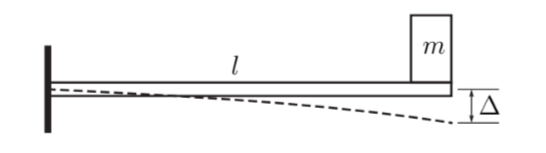
\includegraphics[width=\linewidth]{imgs/mola_eq_1.png}
                        \end{minipage}
                        &
                        $    \Delta = \frac{Pl^3}{3EI}$ 
                        &
                        $   k = \frac{P}{\Delta} = \frac{3EI}{l^3}$ \\ \hline
                        Viga Bi-Apoiada & 
                        \begin{minipage}{.45\textwidth}
                            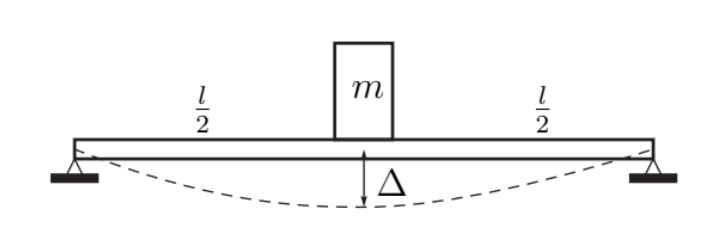
\includegraphics[width=\linewidth]{imgs/mola_eq_2.png}
                        \end{minipage}
                        &
                        $\Delta = \frac{Pl^3}{48EI}$
                        &
                        $k = \frac{P}{\Delta} = \frac{48EI}{l^3}$ \\ \hline 
                        Barra em Solicitação Axial & 
                        \begin{minipage}{.45\textwidth}
                            \centering
                            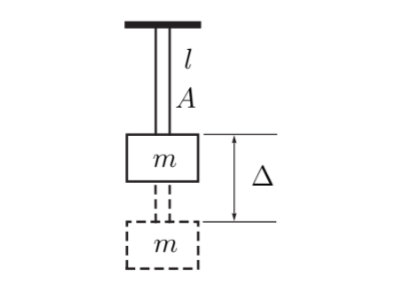
\includegraphics[width=.5\linewidth]{imgs/mola_eq_3.png}
                        \end{minipage}
                        &
                        $\Delta = \frac{Pl}{AE}$
                        &
                        $k = \frac{P}{\Delta} = \frac{AE}{l}$ \\ \hline
                    \end{tabular}
                    \label{tab:molas_equivalentes}
                    \caption{Molas Equivalentes}
                \end{table}

                Onde: 
                \begin{itemize}
                    \item $P$: Força peso, $P = m\cdot g$
                    \item $\Delta$: Deflexão
                    \item $E$: Módulo de Elasticidade
                    \item $I$: Inércia da seção transversal
                \end{itemize}

                \newpage

                Além disso podemos, ainda, ter a associação de molas:
                \begin{table}[h]
                    \centering
                    \begin{tabular}{|c|c|c|c|}
                        \hline
                        Topologia & Diagrama & Equação & Observação \\ \hline
                        Molas em Paralelos
                        &
                        \begin{minipage}{.3\textwidth}
                            \centering
                            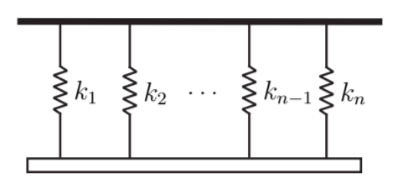
\includegraphics[width=.8\textwidth]{imgs/mola_eq_5.png}
                        \end{minipage}
                        &
                        $k = \sum_{i = 1}^n k_i$
                        &
                        \begin{minipage}{.3\columnwidth}
                            Temos que para molas em paralelo, todas tem o mesmo deslocamento%
                        \end{minipage} \\ \hline

                        Molas Em Série &
                        \begin{minipage}{.3\linewidth}
                            \centering
                            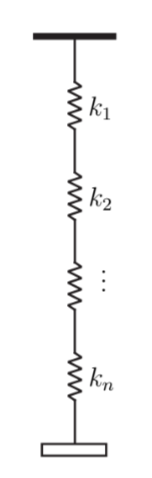
\includegraphics[width=.2\linewidth]{imgs/mola_eq_6.png}
                        \end{minipage}
                        &
                        $k^{-1} = \sum_{i = 1}^n \frac{1}{k_i}$
                        &
                        \begin{minipage}{0.3\columnwidth}
                        Temos que para molas em série, cada uma delas sofre a mesma força. 
                        \end{minipage}\\ \hline
                    \end{tabular}
                    \caption{$k$ Resultante de associação de molas}
                \end{table}

                    
            \subsection{Sistema Torcional}

                \begin{figure}[h]
                    \centering
                    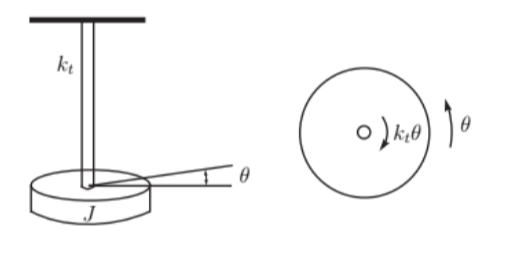
\includegraphics[width=.5\textwidth]{imgs/sis_torcional.png}
                    \caption{Sistema Torcional e $DCL$}
                \end{figure}

                Para introduzirmos um sistema torcinal de vibrações, iremos considerando um sistema de um disco, com um momento de inércia $J$, conectado a um eixo engastado (fixo e sem rotação livre) em uma das suas extremidades, com uma rigidez torcional
                \footnote{Similar à propriedade $k$ de molas normais, mas representa a resistência à torção da mola equivalente, que nesse caso refere-se à viga engastada}
                $k_t$, como mostrado pela figura acima. 

                Quando lidamos com problemas relacionados com rotação, a maioria esmagadora de vezes iremos usar o momento para equacionar o movimento vibracional. Após a análise de corpo livre e
                determinação da coordenada $\theta$ (necessária somente uma pois sistema apresenta somente um grau de liberdade), podemos aplicar a Lei de Newton no que tange momento e temos:

                \begin{align*}
                    \sum M = J \ddot \theta \Rightarrow -k_t\theta = J \ddot \theta
                \end{align*}

                Que pode ser escrita da seguinte forma:

                \begin{align}
                    \ddot\theta + \frac{k_t}{J}\theta = 0 \label{eq:som_moments_sis_torcional}
                \end{align}

                Podemos, então, verificar que, mesmo com uma topologia diferente, o sistema apresenta o mesmo comportamento (e mesma modelagem) do sistema massa mola, com a frequência natura sendo 
                $\omega_n = \sqrt{k_t/J}$

        \section{Vibrações Livres de Sistemas de 1 \emph{DOF} com Amortecimento}

            \subsection{Introdução}
                Até o momento nós vimos situações onde não haviam forças dissipativas atuando sobre o sistema e, por conseguinte, o movimento de vibração continuava eternamente. Isso, entretanto, não
                condiz com a realidade, levando em consideração que há inúmeros mecanismos pelos quais um sistema perde energia. Vários deles, entretanto, podem ser modelados por um 
                \textbf{amortecedor viscoso}, que é regido pela seguinte equação:

                \begin{align}
                    f_d = -c \dot x \label{eq:forca_amortecedor_viscoso}
                \end{align}

                Onde:
                \begin{itemize}
                    \item $c$: Constante do amortecedor
                    \item $\dot x$: A velocidade
                \end{itemize}

                O exemplo mais comum disso é uma massa-mola-amortecedor, como mostrado na figura abaixo:
                \begin{figure}[h]
                    \centering
                    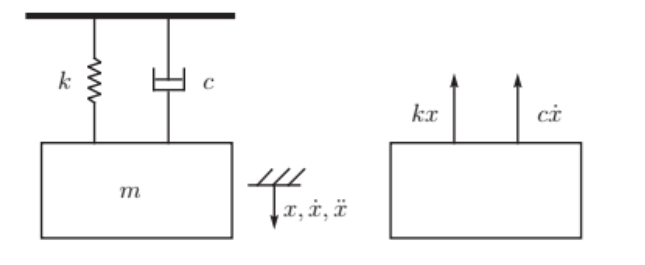
\includegraphics[width=.4\textwidth]{imgs/sis_massa_mola_amortecedor.png}
                    \caption{Sistema Massa-Mola-Amortecedor}
                \end{figure}

                Aplicando a Lei de Newton chegamos em:

                \begin{align}
                    \ddot x + \frac{c}{m}\dot x + \frac{k}{m}x = 0 \label{eq:massa_mola_amortecedor_base}
                \end{align}

                Rotineiramente, entretanto, quando temos um problema com amortecimento nós utilizamos a equação diferencial (que no nosso caso é a equação \ref{eq:massa_mola_amortecedor_base}) da seguinte
                forma:
                \begin{align}
                    \ddot x + 2\zeta \omega_n\dot x + \omega_n^2 x = 0 \label{eq:massa_mola_amortecedor_classica}
                \end{align}

                Onde:
                \begin{itemize}
                    \item $\zeta$: \textbf{Fator de Amortecimento}, parâmetro adimencional que fornece uma medida do amortecimento do sistema (que veremos de forma mais detalhada mais para frente) 
                    \item $\omega_n$: Frequência Natural do sistema, dada por $\sqrt{k/m}$
                \end{itemize}

                \textbf{IMPORTANTE:} Em um sistema amortecido, o sistema \textbf{\emph{NÃO}} oscila com a frequência natural $\omega_n$, mas sim com uma frequência amortecida (também chamada de
                \emph{damped frequency} $\omega_d$, que iremos averiguar mais para frente como é calculada).
                \newpage

            \subsection{Classificação de Sistemas Amortecidos}
                Como vimos anteriormente, podemos modelar um sistema de 1 grau de liberdade amortecido pela equação \ref{eq:massa_mola_amortecedor_classica}, que tem como principal componente que
                descreve o seu amortecimento como sendo o $\zeta$, chamado de fator de amortecimento.
                
                Somos capazes de ver e entender a influência do fator de amortecimento ao analisarmos a equação diferencial característica \ref{eq:massa_mola_amortecedor_classica}, onde, 
                durante a sua resolução (para o qual supomos o sistema com uma resposta $x=Ae^{\lambda t}$), seu polinômio característico\footnote{Importante rever essa parte de Calc III ou Anal, mas o
                polinômio característico é usado para achar o $\lambda$ da exponencial que supomos ser a resposta do sistema} e suas raízes (que regem o comportamento exponencial da resposta) são dadas por:

                \begin{align*}
                    \lambda^2 + 2\zeta \omega_n \lambda + \omega_n^2 = 0 \Rightarrow
                    \lambda_{1,2} = -\zeta \omega_n \pm \omega_n \sqrt{\zeta^2 - 1}
                \end{align*}

                A depender do valor de $\zeta$ temos que o sistema pode ser:
                \begin{itemize}
                    \item $\zeta < 1$: Sub-amortecido
                    \item $\zeta=1$: Criticamente amortecido
                    \item $\zeta > 1$: Super-amortecido
                \end{itemize}

                \subsubsection{Sistema Sub-Amortecido}
                    Dizemos que um sistema é sub-amortecido quando $\zeta < 1$, o que resulta na equação característica ter duas raízes imaginárias tal que:
                    \begin{align}
                        \lambda_{1,2} = \sigma \pm  j \omega_d \Rightarrow \begin{cases}\sigma = -\zeta \omega_n \\ \omega_d = \omega_n \sqrt{1 - \zeta^2}\end{cases}\label{eq:raizes_caso_sub_amortecido}
                    \end{align}
                    
                    Onde a parte imaginária da raiz é chamada de \emph{frequência amortecida} $\omega_d$. 

                    Por fim, teremos como resposta do sistema:
                    \begin{align}
                        x(t) = A_1 e^{\lambda_1 t} + A_2 e^{\lambda_2 t} = e^{-\zeta \omega_n t}(A_1e^{j\omega_dt} + A_2^{-j\omega_d t}) \label{eq:resp_sis_sub_amortecido}
                    \end{align}

                    Onde $A_{1,2}$ são constantes que somos capazes de achar a partir das duas condições iniciais.

                \subsubsection{Sistema Criticamente-Amortecido}
                    Já para quando $\zeta=1$, nós chamamos o sistema de criticamente amortecido, e sua equação característica tem duas raízes reais iguais:
                    \begin{align}
                        \lambda_1 = \lambda_2 = -\zeta \omega_n = -\omega_n \label{eq:raizes_caso_criticamente_amortecido}
                    \end{align}

                     Resultando em uma resposta que \textbf{não oscila} e que é descrita por:
                     \begin{align}
                        x(t) = A_1 e^{-\omega_n t}  + A_2 e^{-\omega_n t}
                     \end{align}

                \subsubsection{Sistema Super-Amortecido}
                     E para o último caso, chamamos de super-amortecido quando $\zeta > 1$, resultando em:






            
\end{document}